We now formally define the problem statement and the technique for retrieving a section title given a book and its Table of Contents ({\toc})

\subsection{Notations}
We are given a long document $D$ and its Table of Contents ${{\toc}}_D = \{T_{1}, T_{2}, ....,T_{n}\}$. An edge $e: T_{p} \rightarrow T_{c}$ between two nodes $T_{p}$, $T_{c}$ $\in {{\toc}}_D$ is defined as $T_{p}$ = parent($T_{c}$), if the section represented by title $T_{p}$ is further divided into multiple sub-sections including $T_{c}$. The set of leaf nodes can thus be defined as $LN_{D}$=$\{T_{l} \in {\toc}_{D} | \exists! T_{c} \in {\toc}_{D}, T_{l}=parent\_of(T_{c})\} \subseteq {{\toc}}_{D}$. Our goal is to retrieve the correct leaf node $T_{l} \in LN_{D}$ whose content can answer a user query $q$.

% Given a long document $D$, we want to search the most relevant content that can answer a user query $q$. Table of Contents, is represented as a tree containing chapter, section and subsection titles.
% ${{\toc}}_D = \{T_{1}, T_{2}, ....,T_{n}\}$. An edge $e: T_{p} \rightarrow T_{c}$ between two nodes $T_{p}$, $T_{c}$ $\in {{\toc}}_D$ is defined as $T_{p}$ = parent($T_{c}$), if the section represented by title $T_{p}$ is further divided into multiple sub-sections including $T_{c}$. The set of leaf nodes can thus be defined as $LN_{D}$=$\{T_{l} \in {\toc}_{D} | \exists! T_{c} \in {\toc}_{D}, T_{l}=parent\_of(T_{c})\} \subseteq {{\toc}}_{D}$. Our goal is to retrieve the correct leaf node $T_{l} \in LN_{D}$ that has the content to answer a user query $q$.

\subsection{Training {\sys}}
\label{subsec:train_task}
% \begin{figure*}[!tbh]
%     \centering
%     % \includegraphics[scale=0.45]{images/arch.png}
%     % \includegraphics[width=\linewidth]{images/system_blue.png}
%     \includegraphics[width=\linewidth]{images/arch.png}
%     \caption{{\sys} Training pipeline}
%     \label{fig:arch}
% \end{figure*}
\begin{figure*}[!tbh]
    \centering
    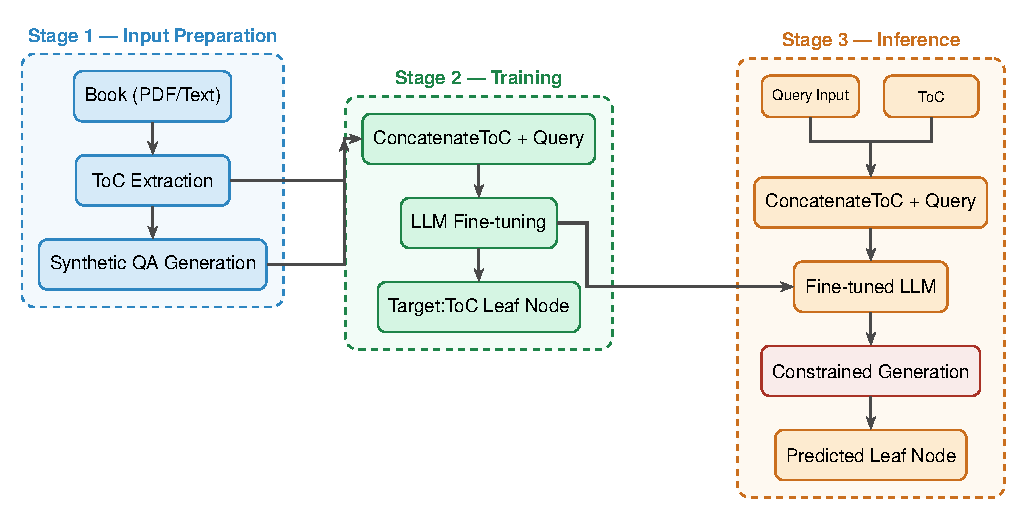
\includegraphics[width=\linewidth]{images/pipeline.pdf}
    \caption{Overview of our pipeline. Stage 1 prepares synthetic QA data
             from the input book. Stage 2 fine-tunes a language model to map
             a ToC-augmented query to the correct leaf node. Stage 3 runs
             inference with constrained generation, restricting the output
             vocabulary to valid ToC leaf nodes.}
    \label{fig:arch}
\end{figure*}
\noindent Figure~\ref{fig:arch} depicts the training pipeline for {\sys} which learns two correlated but \textit{different} tasks:\\
\textbf{Corpus knowledge ingestion:} {\sys} needs to learn the information trove $D$ by mapping a book's text content to the corresponding section titles $T_{i} \in {\toc}_{D}$. This is facilitated by the training data, which consists of a series of queries that are linked to their corresponding section titles. Consequently, this phase of training integrates the book's knowledge into the LLM's parameters, similar to model-based indexing systems like DSI, but with a key difference. Unlike other model-based indexing systems, the parameters in {\sys} remember the corpus knowledge not by a document identifier, but by using fine-grained section title entries in the {\toc}, which are likely to have a much stronger semantic connection with the content being ingested into parametric knowledge.

\textbf{Learning to generate from {\toc}:} {\sys} learns to pick the most relevant leaf node from the complete global structure ({\toc}) of a document.
% \textbf{Learning to generate from {\toc}:} {\sys} learns the implicit task of selecting the most relevant leaf node only from the smaller subset of leaf nodes $LN_{D} \subset {\toc}_{D}$, we implement special demarcations by adding a prefix \textit{leaf} before the section titles when presenting {\toc} as input to it. We also create a prompt that specifically instructs the LLM to choose only from leaf nodes, as shown in Table~\ref{table:train_example_small}. This prompt and the use of leaf node demarcation remain consistent throughout both training and evaluation. During training, the repeated application of the unchanging prompt with identifiable leaf nodes fine-tunes the LLM's generation process, enabling it to align with the new task of generating leaf node {\toc} entries.
 
\eat{In order to help {\sys} learn the implicit task picking only from the smaller subset of leaf nodes $LN_{D} \subset {\toc}_{D}$ we do special demarcations of leaf nodes by including a prefix \textit{leaf} before the section titles while presenting the {\toc} as input to {\sys}. We also create a prompt which specifically asks the LLM to pick only from leaf nodes as shown in Table~\ref{table:train_example_small}. The prompt and the use of leaf node demarcation remains constant through out the training as well as evaluation. During training, the repeated use of unchanging prompt with identifiable leaf nodes tunes the LLM generation such that the LLM learns to align the instruction with this new task of generating leaf node {\toc} entries. Please see Appendix~\ref{sec:appendix_train_example} for a complete training example}

% An example format of how the prompt, instruction and {\toc} are used to train the LLM is shown in Figure~\ref{fig:train_example}.

\eat{
Unlike traditional seq-to-seq training where generations from LLM are trained using gold free text generations, for {\sys} there is an additional task, where it has to learn to generate the correct section title from the available {\toc} which it receives as input. More precisely, it has to be pick a section title which is a leaf node in input {\toc} i.e. $LLM.Generate \in LN_{D} \subset {\toc}_{D}$. This task is very specific to our paradigm and amounts to learning to choose the right option from an input set of options represented in ${\toc}_{D}$. In order to help {\sys} learn the implicit task picking only from the smaller subset of leaf nodes $LN_{D} \subset {\toc}_{D}$ we do special demarcations of leaf nodes by including a prefix \textit{leaf} before the section titles while presenting the {\toc} as input to {\sys}. We also create a prompt which specifically asks the LLM to pick only from leaf nodes as shown in Table~\ref{table:train_example_small}. The prompt and the use of leaf node demarcation remains constant through out the training as well as evaluation. During training, the repeated use of unchanging prompt with identifiable leaf nodes tunes the LLM generation such that the LLM learns to align the instruction with this new task of generating leaf node {\toc} entries. 
% An example format of how the prompt, instruction and {\toc} are used to train the LLM is shown in Figure~\ref{fig:train_example}.
}

\eat{The exact training regime of {\sys} is described below:}

\eat{
ToDo Suggestions(Jaydeep) \\
- have a architecture diagram with seq-to-seq model with specific I/O, then use fig1 as a demonstration. \\
- explain the architecture diagram via notations.
- call out it acts as a joint training for two tasks \\
  -- corpus learning: talk about how the training questions in the benchmark is aimed towards coverage. \\
  -- task learning (pick a leaf node from {\toc}) : how the specific prompt is used across all training examples to teach the model the specific task. \\
- mention that in experiments we will ablate against both these forms of learning.\\
}

\eat{\par{\textbf{Training:}}}
We use the training split from {\ben} to train {\sys} through supervised fine-tuning. During training, we provide the query $q$ along with the complete ${\toc}_{D}$ as input. Consequently, the complete input during training consists of \textit{prompt} + $(q,{\toc}_{D})$. Note that ${\toc}_{D}$, remains consistent across queries from the same book, while the prompt remains unchanged throughout the training process. We fine-tune the model to generate the correct leaf node $T_{l}\in LN_{D}$ that corresponds to the query $q$.

\begin{table}[!htb]
\small
\caption{Sample training example}
\label{table:train_example_small}
\begin{tabular}{l}
\textbf{Prompt} \\
\toprule
\#\#\# Book: Teaching in a Digital Age\\
Pick the best section from the table of contents below\\
which can answer the user query below. Only generate \\
the section name, do not generate any explanation!\\
\\
\#\#\#\ Table of Contents\\
1 Chapter 1: Fundamental Change in Education \\
$\cdots$ \\
leaf 12.7 Step five:master the technology \\
leaf 12.8 Step six:set appropriate learning goals \\
leaf 12.9 Step seven:design course structure and learning\\
$\cdots$ \\
leaf 13.7 Building the future \\
\#\#\# Query: What is the suggested time allocation \\ 
for students studying a course or program? \\
\#\#\# Section: leaf \\
\\
\textbf{Completion} \\
\midrule
12.9 Step seven: design course structure and learning
\end{tabular}
\end{table}